\documentclass[t,9pt]{beamer}

\usetheme{CambridgeUS}
\usecolortheme{seahorse}

\setbeamertemplate{navigation symbols}{}
\setbeamertemplate{section in toc}[ball unnumbered]
\setbeamertemplate{headline}{}
 
\usefonttheme{serif}
\usepackage{newtxmath}
\usepackage[onehalfspacing]{setspace}

% \usepackage[ngerman]{babel}
\usepackage{amsmath,amssymb,amsfonts}
\usepackage{siunitx}
\usepackage[absolute,overlay]{textpos}
\usepackage{bookmark}
\usepackage{csquotes}

\usepackage{caption}
\usepackage{svg}

\usepackage[framemethod=TikZ]{mdframed}
\usepackage{tcolorbox}
\tcbuselibrary{theorems}
\tcbuselibrary{skins}

\newcommand{\td}{\text{d}}

\newcommand{\highlight}[3]{ \begin{textblock*}{#1}(#2,#3) \begin{tcolorbox} [enhanced,opacityfill=.1,colback=blue] \end{tcolorbox} \end{textblock*} } % \highlight{100pt}{10pt}{25pt}

\title[\thesection]{Particle Detectors and Instrumentations}
\subtitle{Observation of Multiple Scattering}
\author{Group 1}
\institute{Universität Bonn}
\date{\today}
%\logo{\LaTeX{}}

\begin{document}

        \iffalse\AddToHook{shipout/foreground}{
          \begin{tikzpicture}[remember picture,overlay]
            \node[red,rotate=30,scale=5,opacity=0.1] at (current page.center) {Draft};
          \end{tikzpicture}
        }\fi

        \begin{frame}
                \titlepage
        \end{frame}

        % \begin{frame}{Inhaltsverzeichnis}
        %         \tableofcontents
        % \end{frame}
        
        \begin{frame}
                \vfill
                \begin{figure}
                        \centering
                        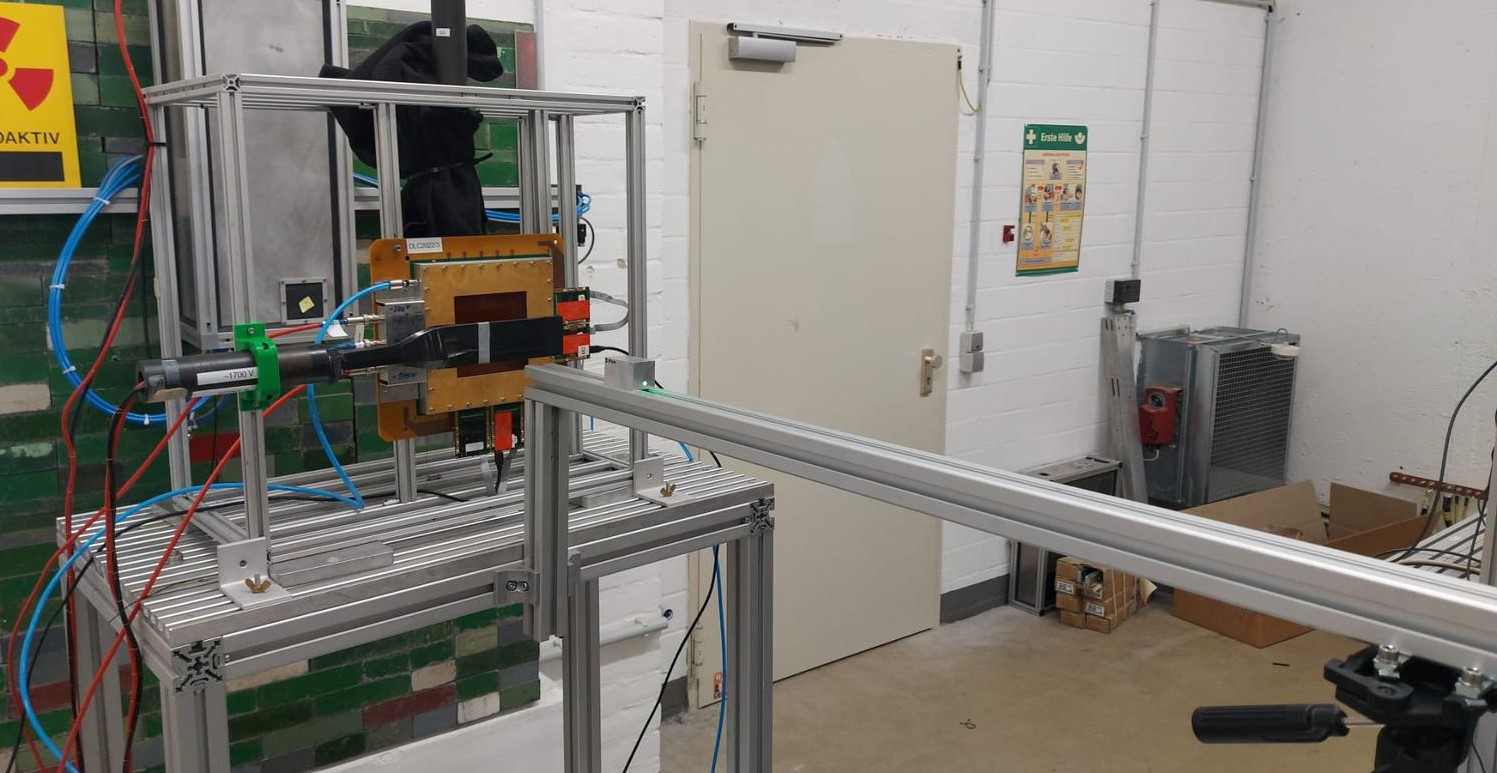
\includegraphics[trim={5cm 0 5cm 0},clip, width=.9\textwidth]{./figures/detector_setup_elsa.jpg}
                        \caption{Setup of experimental site at ELSA.}
                \end{figure}
        \end{frame}

        \begin{frame}
                \vfill
                \begin{figure}
                        \centering
                        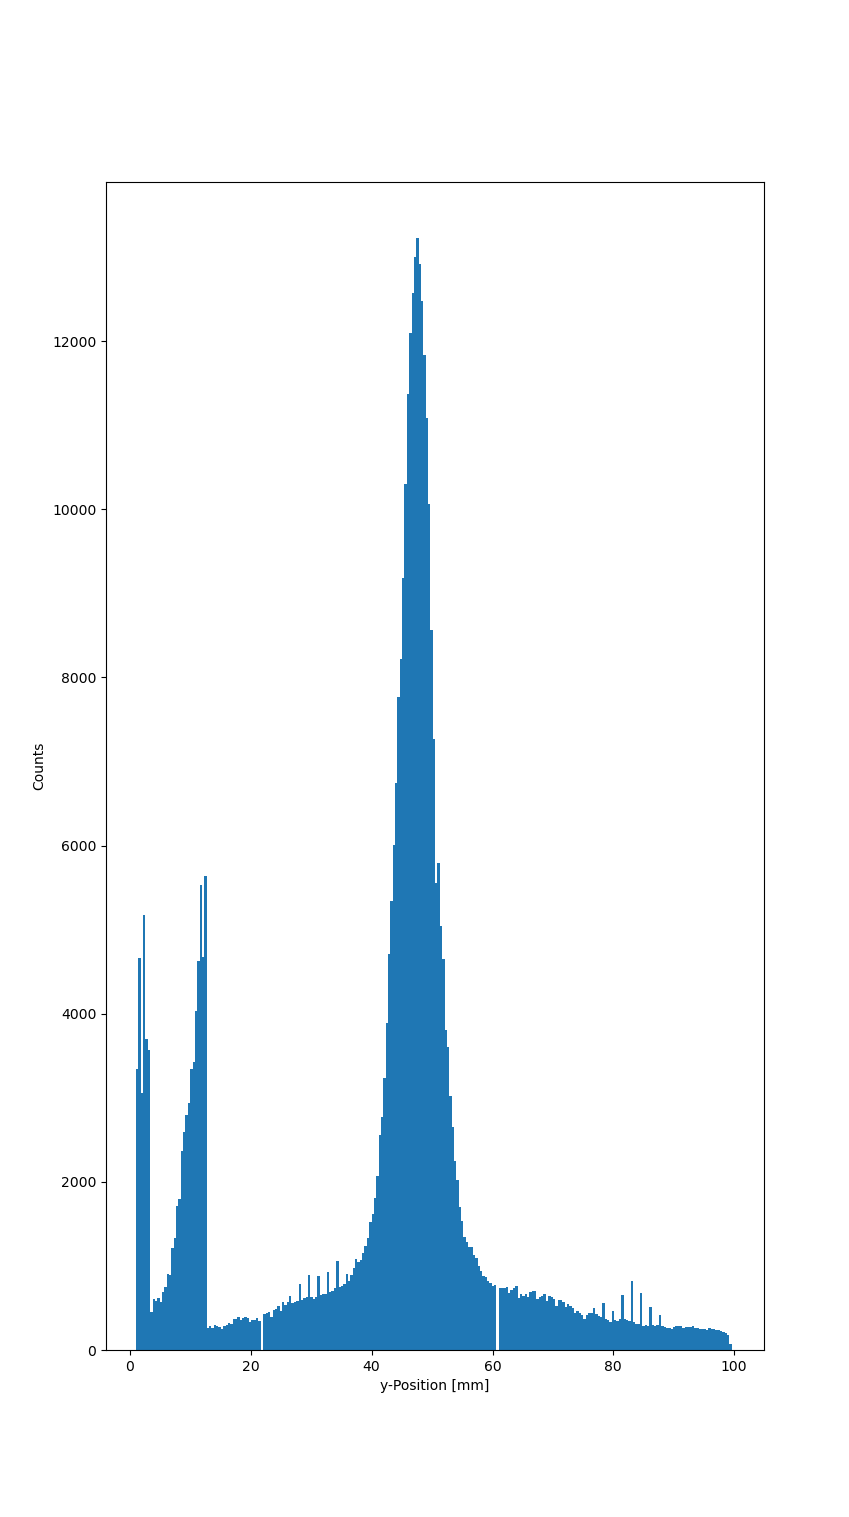
\includegraphics[width=.8\textwidth]{../src/elsa/finished_plots/unfiltered_noMaterial.png}
                        \caption{Raw data of the beam without target.}
                \end{figure}
        \end{frame}

        \begin{frame}
                \vfill
                \begin{figure}
                        \centering
                        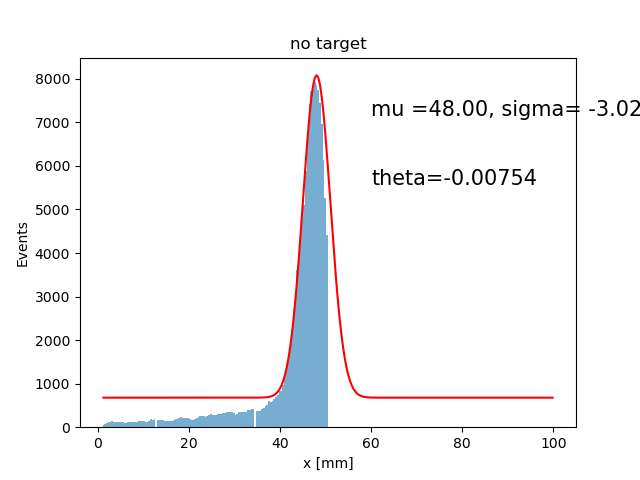
\includegraphics[width=.8\textwidth]{../src/elsa/finished_plots/no target.png}
                        \caption{Filtered beam profile without target.}
                \end{figure}
        \end{frame}

\end{document}